% Capitulo: Do simulador ao carro real -- identificar a planta e reprojetar o controle de velocidade
%
% Figuras e numeros:  simulador/.venv/Scripts/python.exe veiculo_real/capitulo/figuras.py
% Compilar (dentro de veiculo_real/capitulo), duas vezes por causa das referencias:
%   pdflatex -aux-directory=build controle_carro_real.tex
\documentclass[11pt,a4paper,oneside,openany]{book}
\usepackage[utf8]{inputenc}
\usepackage[T1]{fontenc}
\usepackage[brazil]{babel}
\usepackage{lmodern}
\usepackage{microtype}
\usepackage{amsmath,amssymb}
\usepackage{graphicx}
\usepackage{booktabs,array,tabularx}
\usepackage[table]{xcolor}
\usepackage[a4paper,margin=2.4cm]{geometry}
\usepackage[font=small,labelfont=bf]{caption}
\usepackage{listings}
\usepackage[most]{tcolorbox}
\usepackage{tikz}
\usetikzlibrary{arrows.meta,positioning,calc,decorations.pathreplacing}
\usepackage{siunitx}
\sisetup{output-decimal-marker={,}, range-phrase={~a~}, range-units=single}
\usepackage[section]{placeins}
\usepackage{needspace}
\usepackage{hyperref}
\renewcommand{\topfraction}{0.9}
\renewcommand{\bottomfraction}{0.8}
\renewcommand{\textfraction}{0.07}
\renewcommand{\floatpagefraction}{0.75}
\setcounter{topnumber}{3}
\setcounter{totalnumber}{5}

\definecolor{azul}{HTML}{2A78D6}
\definecolor{azulescuro}{HTML}{104281}
\definecolor{laranja}{HTML}{EB6834}
\definecolor{cinza}{HTML}{898781}
\definecolor{tinta2}{HTML}{52514E}
\hypersetup{colorlinks, linkcolor=azulescuro, urlcolor=azulescuro, citecolor=azulescuro}

\newtcolorbox{ideia}{colback=azul!6, colframe=azul, fonttitle=\bfseries\small, title={Ideia-chave}, breakable}
\newtcolorbox{armadilha}{colback=laranja!7, colframe=laranja, fonttitle=\bfseries\small, title={Armadilha}, breakable}
\newtcolorbox{pense}{colback=cinza!8, colframe=cinza, fonttitle=\bfseries\small, title={Pare e pense}, breakable}
\newtcolorbox{caixa}[1]{colback=white, colframe=azulescuro, fonttitle=\bfseries\small, title={#1}, breakable}

\lstset{basicstyle=\ttfamily\footnotesize, keywordstyle=\color{azulescuro}\bfseries,
  commentstyle=\color{cinza}\itshape, stringstyle=\color{laranja}, frame=single,
  rulecolor=\color{cinza!50}, backgroundcolor=\color{cinza!5}, language=Python,
  showstringspaces=false, columns=fullflexible, xleftmargin=2mm, framexleftmargin=1mm,
  aboveskip=6pt, belowskip=6pt}

\graphicspath{{figs/}}
\newcommand{\code}[1]{\texttt{#1}}
\newcommand{\vmed}{v_{\text{med}}}
\newcommand{\Knom}{K_{\text{NOM}}}

\setlength{\parskip}{3pt}

\begin{document}

\chapter{Do simulador ao carro real}

\begin{center}
\itshape Como identificar a planta de verdade a partir dos logs que você já tem\\
e reprojetar o controle de velocidade, sem adivinhar nada.
\end{center}

\bigskip

Você projetou um controlador de velocidade no simulador. Ele foi identificado com
cuidado, validado com previsão cega, e funcionava. Copiou para o carro real, rodou,
e o carro disparou: com referência de \SI{1}{m/s}, ficou andando a \SI{1,85}{m/s}
durante o ensaio inteiro, e o controlador não fez nada para corrigir.

Este capítulo é a investigação desse problema, do começo ao fim, com o raciocínio
explícito em cada passo. Não há nada aqui que exija genialidade: há um método. Cada
passo responde a uma pergunta, e cada resposta vem de uma fonte que você consegue
conferir --- o código, a física ou os dados.

\begin{caixa}{O que você vai aprender}
\begin{enumerate}\itemsep0pt
  \item Ler o código antes dos dados, para descobrir a \emph{estrutura} da planta.
  \item Modelar só o que o código não diz, com poucos parâmetros e significado físico.
  \item Fazer inventário e triagem dos logs, descartando com evidência.
  \item Reconstruir sinais que não foram medidos.
  \item Ajustar o modelo pela trajetória inteira (erro de saída).
  \item Validar: testes físicos, previsão cega e o que os dados \emph{não} conseguem dizer.
  \item Descobrir, pelos próprios logs, que código estava rodando.
  \item Montar um simulador do carro real e validá-lo contra os ensaios.
  \item Projetar o controlador: estrutura, ganho nominal e ganho proporcional.
\end{enumerate}
\end{caixa}

% ---------------------------------------------------------------------------
\section{O sintoma}

O controlador que rodou no carro é o do simulador: um PI com
\emph{feedforward} da referência, compensação do atrito identificado
($a_0 = \SI{0,096}{m/s^2}$, $c = \SI{0,00425}{1/m}$), um filtro passa-baixas no
comando e saturação $u \in [0,\,1]$. No simulador, a planta identificada era
\begin{equation}
  \dot v = K u - c\, v|v| - a_0\,\mathrm{sign}(v), \qquad K \approx 1{,}0,
  \label{eq:planta-sim}
\end{equation}
ou seja, $u$ era uma \emph{aceleração}: com $u=0$, o atrito freava o carro.

Nos ensaios do carro real (24/09, carro roxo), o comportamento foi outro:

\begin{center}
\begin{tabular}{lcc}
\toprule
referência & velocidade em regime & quanto tempo ficou lá\\
\midrule
\SI{1,0}{m/s} & \SIrange{1,74}{1,87}{m/s} & até o fim do ensaio\\
\SI{0,5}{m/s} & \SIrange{1,31}{1,41}{m/s} & até o fim do ensaio\\
\bottomrule
\end{tabular}
\end{center}

E durante todo esse tempo o comando ficou em $u = 0$.

\begin{pense}
Se $u$ fosse aceleração, como na equação~\eqref{eq:planta-sim}, o que deveria acontecer
com um carro a \SI{1,85}{m/s} e $u = 0$ durante \SI{17}{s}? E o que os logs mostram?
A diferença entre as duas respostas é a pista de que a planta do carro real não é a do
simulador.
\end{pense}

% ---------------------------------------------------------------------------
\section{Passo 1: leia o código antes dos dados}

A primeira tentação é abrir os logs e ajustar a equação~\eqref{eq:planta-sim} de novo.
Resista. Antes de olhar dado, descubra \emph{o que o sinal $u$ faz} até chegar à roda.
Essa informação está no código, e o código não tem ruído.

\subsection{O caminho do comando}

O controlador chama \code{car.set\_u(u)}. Seguindo a chamada:

\begin{lstlisting}[title={\small\code{veiculo\_real/fva\_car/car.py}}]
def set_u(self, u):
    self.u = np.clip(u, -CAR['ACCELMAX'], CAR['ACCELMAX'])   # u em [-1, 1]
    if np.abs(self.v) > CAR['VELMAX']:
        self.u = 0.0
    F = CAR['MASS']*self.u          # "controlador linearizante"
    T = CAR['RW']*np.sum(F)         # pseudo-torque
    self.atuador.set_torque(T)
\end{lstlisting}

\begin{lstlisting}[title={\small\code{veiculo\_real/fva\_car/servos.py}}]
GAIN_TORQUE_FORWARD = 0.4   # [rad/s] por unidade de pseudo-torque

def set_torque(self, T):
    self.dth_pwm = self.gain_torque * T      # T vira uma TAXA de PWM

# thread "actuator", a cada self.dt = 0.03 s:
if self.gear == Gear.FORWARD:
    self.th_pwm += self.dth_pwm * self.dt                          # integra
    self.th_pwm = np.clip(self.th_pwm, 0.0, self.max_throttle)     # 0 a 18,1 graus
\end{lstlisting}

A linha decisiva é \code{self.th\_pwm += self.dth\_pwm * self.dt}. O comando não vira
um torque nem uma aceleração: vira a \emph{taxa de variação} do PWM do acelerador, e uma
thread separada integra essa taxa. Juntando as constantes ($m = \SI{5,16}{kg}$,
$R_W = \SI{0,08}{m}$, ganho $0{,}4$):
\begin{equation}
  \dot\theta = k_\theta\, u, \qquad k_\theta = 0{,}4 \cdot 0{,}08 \cdot 5{,}16
  = \SI{0,165}{rad/s} = 9{,}46^\circ\!/\mathrm{s} \text{ por unidade de } u,
  \label{eq:integrador}
\end{equation}
com $\theta$ (o PWM acima do neutro) limitado a $[0^\circ,\,18{,}1^\circ]$.

\begin{ideia}
O nome de uma variável não diz o que ela faz; o código diz. No simulador, $u$ era
aceleração. No carro real, $u$ é a \emph{velocidade com que o acelerador anda}. Isso
coloca um integrador puro entre o controlador e o motor, antes de qualquer física do
carro. Com $u = 0$, o acelerador fica parado onde está --- e o carro mantém a velocidade.
\end{ideia}

\begin{caixa}{É possível ter $u$ negativo no carro real?}
Sim. O \code{set\_u} aceita $u \in [-1,\,1]$, o \code{set\_torque} repassa o sinal, e a
thread subtrai do PWM. O que $u<0$ \emph{faz} fisicamente é o que importa:
\begin{itemize}\itemsep0pt
  \item \textbf{baixa o acelerador}, até o neutro ($\theta = 0$) e não além: em marcha
    à frente a thread limita $\theta \ge 0$. Não é freio nem ré --- é tirar o pé do
    acelerador e deixar o carro ir no embalo. A ré exige \code{set\_reverse()}, um
    procedimento de \SI{5}{s} que o \code{set\_u} nunca chama;
  \item \textbf{o próprio código do professor usa $u<0$}: o PD do \code{set\_vel} dá
    $u<0$ sempre que $v > v_{\text{ref}}$, e o \code{stop\_mission} aplica
    $u = -1$ para parar;
  \item \textbf{os logs confirmam} (Seção~\ref{sec:desce}): no ensaio 003552, a parada
    do ultrassom levou $u$ a $-0{,}68$, o PWM reconstruído caiu de $18{,}1^\circ$ para
    $9{,}3^\circ$ e o carro desacelerou de 1,5 para \SI{0,9}{m/s}.
\end{itemize}
O limite físico: para desacelerar, o carro depende do atrito (embalo), então desacelera
mais devagar do que acelera. Isso entra no projeto como um caso de robustez.
\end{caixa}

\subsection{O caminho da medição}

A velocidade que o controlador enxerga também tem uma história:
\begin{itemize}\itemsep0pt
  \item o \textbf{encoder} (firmware \code{odometer.ino}) conta pulsos em janelas de
    \SI{30}{ms} e manda um valor por janela, com sinal (quadratura);
  \item o \code{car.py} passa esse valor por uma \textbf{média móvel de 30 amostras}
    (\code{MovingAverage(n=30)}), que chamaremos de MA30:
  \begin{equation}
    \vmed[k] = \frac{1}{N}\sum_{i=0}^{N-1} v_{\text{enc}}[k-i], \qquad N = 30.
  \end{equation}
\end{itemize}

Uma média de $N$ amostras espaçadas de $T$ tem fase linear na frequência: ela atrasa o
sinal de
\begin{equation}
  \text{atraso de grupo} = \frac{N-1}{2}\,T.
  \label{eq:atraso-ma}
\end{equation}
Esse atraso depende de $T$, o período do laço. E o período não é o que o código promete.

\subsection{O relógio do laço}

O \code{step()} dorme até completar \SI{20}{ms} desde a última leitura e só
\emph{depois} lê os sensores (encoder, IMU), o que leva cerca de \SI{9}{ms}. O período
real é a soma. A Figura~\ref{fig:dt} mostra a distribuição medida nos 15 logs: mediana
de \SI{28,8}{ms}, com 5\% das amostras acima de \SI{46}{ms}. Com
$T = \SI{28,8}{ms}$, a equação~\eqref{eq:atraso-ma} dá \SI{0,42}{s} de atraso só na
média móvel --- mais de oito vezes o atraso de \SI{0,05}{s} que o projeto do simulador
assumia.

\begin{figure}[ht]
  \centering
  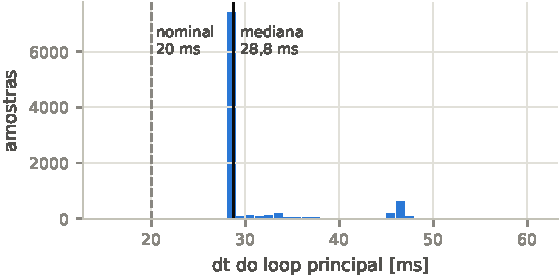
\includegraphics{dt_loop}
  \caption{Período do laço principal nos 15 ensaios. O código pede \SI{20}{ms}; a leitura
  dos sensores vem depois da espera e soma cerca de \SI{9}{ms}.}
  \label{fig:dt}
\end{figure}

A Figura~\ref{fig:laco} mostra a ordem das operações em cada iteração. Ela é importante
para interpretar o log: a linha $k$ é gravada \emph{antes} de o controle calcular o novo
comando, então o $u$ gravado na linha $k$ é o que agiu sobre o carro entre $t_{k-1}$ e
$t_k$.

\begin{figure}[ht]
\centering
\begin{tikzpicture}[font=\scriptsize,
  bx/.style={draw=cinza, fill=cinza!8, minimum height=8mm, align=center, inner sep=2pt},
  cx/.style={bx, draw=azul, fill=azul!10},
  gx/.style={bx, draw=laranja, fill=laranja!12}]
  \node[bx, minimum width=17mm] (s1) at (0,0) {dorme até\\\SI{20}{ms}};
  \node[bx, minimum width=15mm, right=0mm of s1] (r1) {lê sensores\\($\approx$\SI{9}{ms})};
  \node[gx, minimum width=15mm, right=0mm of r1] (w1) {grava linha\\$k-1$};
  \node[cx, minimum width=15mm, right=0mm of w1] (c1) {calcula e\\aplica $u_{k-1}$};
  \node[bx, minimum width=17mm, right=0mm of c1] (s2) {dorme até\\\SI{20}{ms}};
  \node[bx, minimum width=15mm, right=0mm of s2] (r2) {lê sensores\\($\approx$\SI{9}{ms})};
  \node[gx, minimum width=21mm, right=0mm of r2] (w2) {grava linha $k$:\\$t_k$, $v_k$ e $u_{k-1}$};
  \node[cx, minimum width=15mm, right=0mm of w2] (c2) {calcula e\\aplica $u_k$};
  \draw[-{Stealth}, cinza] ([yshift=-4mm]s1.south west) -- ([yshift=-4mm]c2.south east) node[right, black] {tempo};
  \foreach \n/\l in {r1/{t_{k-1}}, r2/{t_k}} {
    \draw ([yshift=-3mm]\n.south east) -- ([yshift=-5mm]\n.south east) node[below] {$\l$};
  }
  \draw[decorate, decoration={brace, mirror, amplitude=5pt}]
    ([yshift=-10mm]r1.south east) -- ([yshift=-10mm]r2.south east)
    node[midway, below=6pt, align=center] {$u_{k-1}$ age sobre o carro neste intervalo\\
    e é o valor gravado na linha $k$};
\end{tikzpicture}
\caption{Duas iterações do laço principal. O instante $t_k$ é carimbado ao fim da leitura
dos sensores.}
\label{fig:laco}
\end{figure}

% ---------------------------------------------------------------------------
\section{Passo 2: modele só o que o código não diz}

O código determinou o começo e o fim da cadeia: o integrador do PWM e a média móvel. O
que fica no meio --- como o PWM vira velocidade --- depende do ESC, do motor, da bateria e
do chão, e isso o código não sabe. É aqui, e só aqui, que entram parâmetros a identificar.

A escolha da estrutura vem da física de um motor CC:
\begin{itemize}\itemsep0pt
  \item \textbf{ganho estático com zona morta.} Em regime, a velocidade de um motor CC é
    proporcional à tensão aplicada, e o PWM define essa tensão. Mas o ESC tem uma faixa
    morta perto do neutro, em que o motor não gira. O próprio \code{servos.py} traz uma
    calibração com essa forma (uma reta com \emph{offset}). Então
    $v_{ss} = G\,\max(0,\ \theta - DB)$;
  \item \textbf{atraso de primeira ordem.} A inércia do motor e do carro faz a velocidade
    chegar ao valor de regime exponencialmente, com constante de tempo mecânica $\tau$;
  \item \textbf{atraso puro $d$.} A janela do encoder e a leitura serial.
\end{itemize}

\begin{caixa}{Modelo do carro real}
\vspace{-2mm}
\begin{align}
  \dot\theta &= k_\theta\,u, && \theta\in[0^\circ,\,18{,}1^\circ] && \text{(código)}\nonumber\\
  v_{ss} &= G\,\max(0,\ \theta - DB) && && \text{(a identificar)}\nonumber\\
  \tau\,\dot v &= v_{ss} - v && && \text{(a identificar)}\label{eq:modelo-real}\\
  \vmed &= \mathrm{MA30}\big(v(t-d)\big) && && \text{(código + a identificar)}\nonumber
\end{align}
Quatro parâmetros livres: $G$, $DB$, $\tau$ e $d$.
\end{caixa}

A Figura~\ref{fig:cadeia} junta tudo. Em azul, o que veio do código; em laranja, o que
precisa sair dos dados.

\begin{figure}[ht]
\centering
\begin{tikzpicture}[>={Stealth}, node distance=4mm and 5mm, font=\footnotesize,
  cod/.style={draw=azul, fill=azul!10, rounded corners=2pt, align=center, minimum height=12mm, inner sep=3pt},
  idt/.style={draw=laranja, fill=laranja!12, rounded corners=2pt, align=center, minimum height=12mm, inner sep=3pt}]
  \node (u) {$u$};
  \node[cod, right=of u] (m) {$F = m\,u$\\$T = R_W F$\\\scriptsize\code{set\_u}};
  \node[cod, right=of m] (g) {$\dot\theta = 0{,}4\,T$\\\scriptsize\code{set\_torque}};
  \node[cod, right=of g] (i) {$\displaystyle\int\!dt$, limite\\$0$ a $18{,}1^\circ$\\\scriptsize thread \code{actuator}};
  \node[right=of i] (th) {$\theta$};
  \draw[->] (u) -- (m); \draw[->] (m) -- (g); \draw[->] (g) -- (i); \draw[->] (i) -- (th);
  \node[idt, below=14mm of m.south west, anchor=north west] (esc) {$G\max(0,\theta-DB)$\\\scriptsize ESC + motor + chão};
  \node[idt, right=8mm of esc] (lag) {$\dfrac{1}{\tau s+1}$\\\scriptsize inércia};
  \node[idt, right=8mm of lag] (enc) {$e^{-ds}$\\\scriptsize encoder};
  \node[cod, right=8mm of enc] (ma) {média de 30\\\scriptsize\code{car.py}};
  \node[right=of ma] (vm) {$\vmed$};
  \draw[->] (th.south) -- ++(0,-9mm) -| (esc.north);
  \draw[->] (esc) -- node[above] {$v_{ss}$} (lag);
  \draw[->] (lag) -- node[above] {$v$} (enc);
  \draw[->] (enc) -- (ma);
  \draw[->] (ma) -- (vm);
  \node[cod, minimum height=4mm, below=6mm of esc.south west, anchor=north west, font=\scriptsize] (l1) {vem do código};
  \node[idt, minimum height=4mm, right=3mm of l1, font=\scriptsize] {a identificar nos dados};
\end{tikzpicture}
\caption{A cadeia do comando até a velocidade medida no carro real.}
\label{fig:cadeia}
\end{figure}

\begin{armadilha}
Não escolha a estrutura pelo ajuste. Um modelo com mais termos sempre ajusta melhor, mas
só a estrutura certa \emph{prevê}. Aqui a estrutura veio do código (integrador, média
móvel) e da física (ganho, zona morta, inércia); o ajuste só dá os números.
\end{armadilha}

% ---------------------------------------------------------------------------
\section{Passo 3: inventário e triagem dos dados}

Havia quatro pastas de logs. A primeira verificação foi um \emph{hash} (md5) de cada
arquivo: as pastas eram cópias cumulativas umas das outras, com arquivos idênticos. No
total, 15 ensaios distintos, todos de \SI{20}{s}.

Nem todo ensaio tem informação sobre a planta. Um ensaio só serve para identificar se o
carro de fato respondeu ao comando. Para decidir isso sem achismo, há uma testemunha
independente do encoder: a IMU. Um carro parado tem aceleração medida quase constante; um
carro andando ou sendo carregado na mão, não (Figura~\ref{fig:imu}).

\begin{figure}[ht]
  \centering
  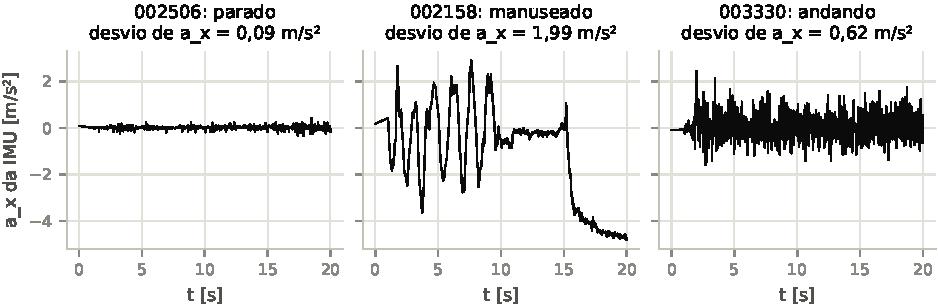
\includegraphics{triagem_imu}
  \caption{A IMU como testemunha. No 002506, $u = 1$ por \SI{18,7}{s} e a IMU não se
  mexe: o motor não respondeu (bateria fraca). No 002158, o encoder marca zero, mas a IMU
  está agitada: o carro estava sendo manuseado. No 003330, o carro andou.}
  \label{fig:imu}
\end{figure}

\begin{table}[ht]
\centering\small
\caption{Triagem dos 15 ensaios. O desvio padrão de $a_x$ (IMU) separa carro parado
($\approx$\SI{0,1}{m/s^2}) de carro em movimento ou manuseado.}
\label{tab:triagem}
\begin{tabular}{llrrrrl}
\toprule
ensaio & hora & $\max|v|$ & $u$ (mín / máx) & $v_{\text{ref}}$ máx & desvio $a_x$ & classificação\\
\midrule
000844 & 00:08 & 0,16 & 0,00 / 0,30 & 0,70 & 0,50 & código do professor\\
002158 & 00:21 & 0,00 & $-$0,04 / 1,00 & 1,00 & 1,99 & manuseado\\
002236 & 00:22 & 0,36 & $-$0,11 / 1,00 & 1,00 & 1,24 & manuseado\\
002318 & 00:23 & 0,01 & $-$0,03 / 1,00 & 1,00 & 0,63 & manuseado\\
002506 & 00:25 & 0,00 & 0,00 / 1,00 & 1,00 & 0,09 & parado (bateria fraca)\\
\rowcolor{azul!6}002634 & 00:26 & 1,84 & 0,00 / 1,00 & 1,00 & 0,56 & bateria boa\\
\rowcolor{azul!6}002751 & 00:27 & 1,87 & 0,00 / 1,00 & 1,00 & 0,50 & bateria boa\\
003019 & 00:30 & 0,00 & 0,00 / 0,00 & 0,00 & 0,08 & parada do ultrassom\\
003157 & 00:31 & 0,00 & 0,00 / 0,00 & 0,00 & 0,06 & parada do ultrassom\\
003238 & 00:32 & 0,00 & $-$0,01 / 1,00 & 0,95 & 0,09 & parada do ultrassom\\
\rowcolor{azul!6}003330 & 00:33 & 1,87 & 0,00 / 1,00 & 1,00 & 0,62 & bateria boa\\
\rowcolor{azul!6}003552 & 00:35 & 1,51 & $-$0,68 / 1,00 & 1,00 & 0,89 & descarregando\\
\rowcolor{azul!6}003904 & 00:39 & 1,78 & 0,00 / 1,00 & 1,00 & 1,41 & descarregando\\
\rowcolor{azul!6}004516 & 00:45 & 1,35 & 0,00 / 1,00 & 0,50 & 1,26 & descarregando\\
\rowcolor{azul!6}004851 & 00:48 & 1,41 & 0,00 / 1,00 & 0,50 & 1,41 & descarregando\\
\bottomrule
\end{tabular}
\end{table}

A Tabela~\ref{tab:triagem} mostra o resultado. Os ensaios destacados (sete) são os que
servem para identificar; cada descarte tem uma evidência na própria tabela:
\begin{itemize}\itemsep0pt
  \item \textbf{000844}: $u$ máximo de $0{,}30 = 0{,}4 \times 0{,}7$, exatamente o PD do
    \code{set\_vel(0,7)} do professor. Não era o controlador em estudo;
  \item \textbf{002506}: $u = 1$ e a IMU parada: o motor não respondeu (bateria fraca);
  \item \textbf{002158, 002236, 002318}: IMU agitada sem leitura coerente do encoder:
    manuseio;
  \item \textbf{003019, 003157, 003238}: $v_{\text{ref}} = 0$ quase o tempo todo: a
    parada por obstáculo do ultrassom estava ativa.
\end{itemize}

\begin{ideia}
Descartar exige evidência. Um log descartado ``porque ficou estranho'' é um viés que você
colocou no modelo. Um log descartado porque a IMU prova que o carro estava parado com
$u = 1$ é informação: ele diz que, naquele momento, o motor não estava sendo alimentado.
\end{ideia}

% ---------------------------------------------------------------------------
\section{Passo 4: reconstrua o que não foi medido}

O PWM do acelerador, $\theta$, não é gravado. Mas o código diz exatamente como ele é
calculado (equação~\eqref{eq:integrador}), e o $u$ que o alimenta está no log. Então
dá para refazê-lo, integrando $u$ como a thread faz, com o limite de
$0^\circ$ a $18{,}1^\circ$ e respeitando a ordem da Figura~\ref{fig:laco}:
\begin{equation}
  \theta_k = \mathrm{clip}\big(\theta_{k-1} + k_\theta\, u_k\,(t_k - t_{k-1}),\ 0,\ 18{,}1^\circ\big).
\end{equation}

A Figura~\ref{fig:pwm} mostra o resultado para o ensaio 003330. Enquanto $u = 1$, o PWM
sobe a $9{,}46^\circ$ por segundo; quando $u$ cai para zero, o PWM \emph{congela} em
$14{,}3^\circ$ (79\% do limite). A velocidade segue o PWM com atraso e fica em
\SI{1,85}{m/s}.

\begin{figure}[ht]
  \centering
  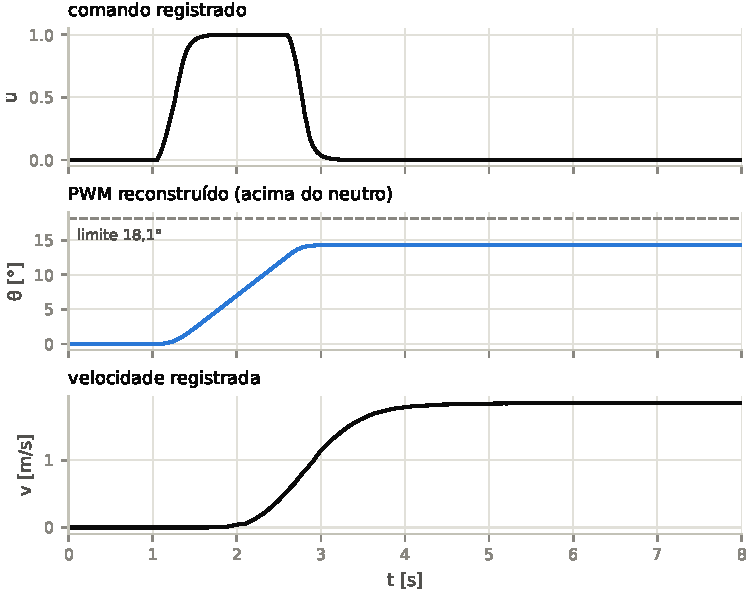
\includegraphics{pwm_reconstruido}
  \caption{Ensaio 003330. De cima para baixo: o comando registrado, o PWM reconstruído
  pela integração do código e a velocidade registrada. Com $u = 0$, o acelerador fica
  parado --- e o carro também fica na mesma velocidade.}
  \label{fig:pwm}
\end{figure}

Aqui o sintoma do início do capítulo se explica sozinho: o controlador só podia mandar
$u \ge 0$. Quando o carro passou da referência, o melhor que ele conseguia fazer era
$u = 0$ --- que, neste carro, significa \emph{manter o acelerador}. É uma catraca: o PWM
só sobe.

% ---------------------------------------------------------------------------
\section{Passo 5: ajuste pela trajetória inteira}

Há duas formas de ajustar um modelo dinâmico a dados:
\begin{itemize}\itemsep0pt
  \item \textbf{erro de equação}: estimar $\dot v$ a partir dos dados e ajustar a equação
    amostra a amostra, usando a velocidade \emph{medida} em cada passo. É fácil de
    resolver (mínimos quadrados lineares), mas é um teste fácil de passar: o erro de um
    passo não se propaga para o próximo;
  \item \textbf{erro de saída}: dar ao modelo \emph{só} o comando registrado, simular o
    ensaio inteiro e comparar a trajetória simulada com a registrada. O erro se acumula,
    então o modelo precisa acertar a dinâmica, não só a derivada.
\end{itemize}

Aqui usamos erro de saída, pelo mesmo motivo do \code{IDENTIFICACAO.md} (§7): é o
critério que corresponde ao uso do modelo --- prever o que o carro vai fazer. O custo é
\begin{equation}
  J(G, DB, \tau, d) = \sum_k \big(\hat v_k(G, DB, \tau, d) - v_k\big)^2,
\end{equation}
em que $\hat v_k$ é a saída do modelo~\eqref{eq:modelo-real} simulado a partir do $u$
registrado, passando pela mesma média de 30 amostras. Como $\hat v$ depende dos parâmetros
de forma não linear (zona morta, exponencial, limites), o mínimo é encontrado por mínimos
quadrados não lineares (função \code{least\_squares} do \code{scipy}), com limites físicos para
cada parâmetro ($G > 0$, $DB \ge 0$, $\tau > 0$, $d \ge 0$).

\begin{table}[ht]
\centering\small
\caption{Parâmetros ajustados por ensaio. $K = G\cdot\frac{180}{\pi}\cdot k_\theta$ é o
ganho do integrador visto pelo controlador, em m/s$^2$ por unidade de $u$.}
\label{tab:param}
\begin{tabular}{llccccc c}
\toprule
ensaio & hora & $G$ [m/s/°] & $DB$ [°] & $\tau$ [s] & $d$ [s] & $K$ & rmse [m/s]\\
\midrule
002634 & 00:26 & 0,158 & 3,03 & 0,289 & 0,000 & 1,49 & 0,009\\
002751 & 00:27 & 0,169 & 3,49 & 0,259 & 0,000 & 1,60 & 0,011\\
003330 & 00:33 & 0,170 & 3,42 & 0,251 & 0,000 & 1,61 & 0,009\\
\midrule
003552 & 00:35 & 0,113 & 2,31 & 0,760 & 0,049 & 1,07 & 0,016\\
003904 & 00:39 & 0,112 & 2,52 & 0,749 & 0,000 & 1,06 & 0,017\\
004516 & 00:45 & 0,093 & 1,11 & 0,634 & 0,000 & 0,88 & 0,014\\
004851 & 00:48 & 0,099 & 1,76 & 0,616 & 0,000 & 0,93 & 0,025\\
\bottomrule
\end{tabular}
\end{table}

A Tabela~\ref{tab:param} e a Figura~\ref{fig:ajustes} mostram o resultado: o modelo
acompanha as trajetórias com erro de 1 a \SI{2,5}{cm/s}. A última coluna de parâmetros
merece atenção: $K$ é o número que o controlador vai precisar, porque é ele que diz
``quanta aceleração cada unidade de $u$ produz'':
\begin{equation}
  K = G\cdot\frac{180}{\pi}\cdot k_\theta
  \quad\Big[\tfrac{\text{m/s}}{\text{grau}}\cdot\tfrac{\text{grau}}{\text{rad}}\cdot
  \tfrac{\text{rad/s}}{u} = \tfrac{\text{m/s}^2}{u}\Big].
\end{equation}

\begin{figure}[ht]
  \centering
  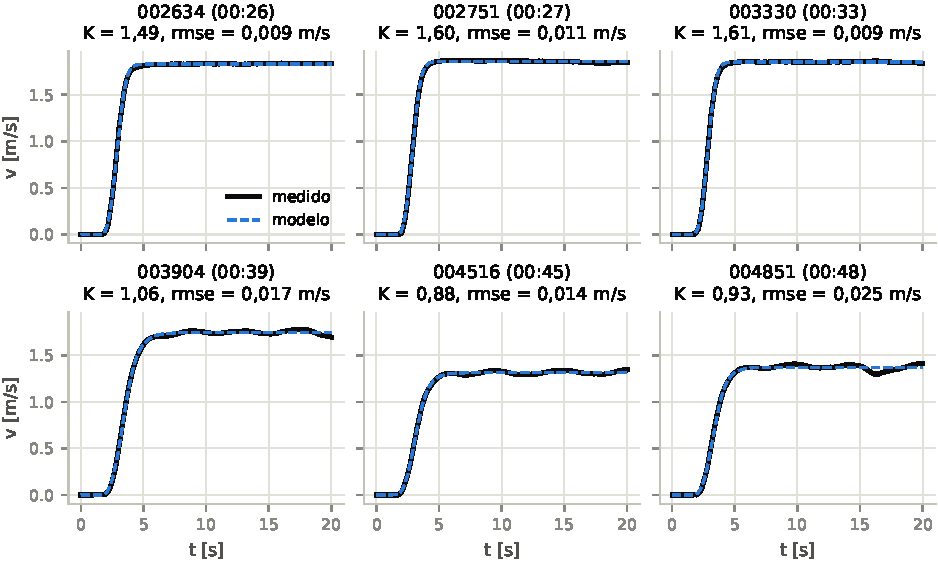
\includegraphics{ajustes}
  \caption{Ajuste por erro de saída em seis ensaios: velocidade medida (preto) e modelo
  simulado só a partir do $u$ registrado (azul tracejado).}
  \label{fig:ajustes}
\end{figure}

% ---------------------------------------------------------------------------
\section{Passo 6: validar é mais importante que ajustar}

Um bom ajuste não prova que o modelo está certo. Três perguntas diferentes precisam de
resposta: o modelo tem a física certa? Ele prevê o que não viu? E o que os dados
\emph{não} conseguem determinar?

\subsection{Com $u = 0$, a velocidade fica parada}

A diferença mais importante entre a planta do simulador~\eqref{eq:planta-sim} e a do carro
real~\eqref{eq:modelo-real} aparece quando $u = 0$. No simulador, o carro desacelera
$a_0 + c\,v^2 \approx \SI{0,11}{m/s^2}$. No modelo real, o PWM congela e a velocidade fica
constante. Os logs decidem:

\begin{center}\small
\begin{tabular}{lccc}
\toprule
ensaio & velocidade com $u=0$ & $\dot v$ medido & $\dot v$ pelo modelo do simulador\\
\midrule
002634 & \SI{1,83}{m/s} & $+0{,}0007$ & $-0{,}110$\\
002751 & \SI{1,86}{m/s} & $-0{,}0020$ & $-0{,}111$\\
003330 & \SI{1,85}{m/s} & $-0{,}0002$ & $-0{,}111$\\
003904 & \SI{1,74}{m/s} & $+0{,}0013$ & $-0{,}109$\\
004516 & \SI{1,31}{m/s} & $+0{,}0011$ & $-0{,}103$\\
004851 & \SI{1,37}{m/s} & $-0{,}0015$ & $-0{,}104$\\
\bottomrule
\end{tabular}
\end{center}

A Figura~\ref{fig:mesmou} mostra o mesmo teste de forma visual: o mesmo $u$ aplicado às
duas plantas. O modelo do simulador pararia o carro em $t \approx \SI{16}{s}$; o carro
real ficou a \SI{1,85}{m/s}, e o modelo identificado acompanha.

\begin{figure}[ht]
  \centering
  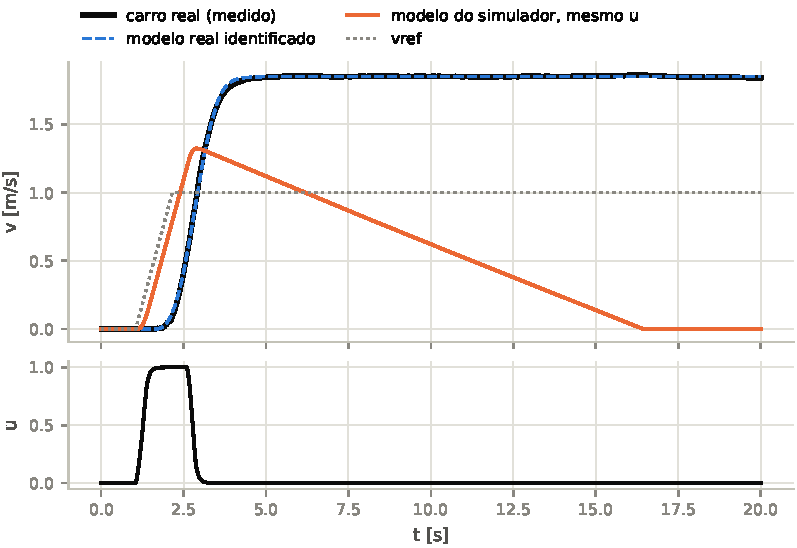
\includegraphics{mesmo_u}
  \caption{Ensaio 003330: o mesmo comando aplicado ao modelo do simulador (laranja) e ao
  modelo identificado do carro real (azul). Só o segundo explica o que o carro fez.}
  \label{fig:mesmou}
\end{figure}

\subsection{O acelerador também desce}
\label{sec:desce}

Em quase todos os ensaios o PWM só subiu, porque o controlador não mandava $u < 0$. Um
modelo validado só com o acelerador subindo não prova que o integrador funciona para
baixo. O ensaio 003552 é a exceção: a parada do ultrassom chamou o \code{set\_vel(0)}, que
mandou $u$ até $-0{,}68$. A Figura~\ref{fig:desce} mostra que o PWM reconstruído desceu, a
velocidade caiu de 1,5 para \SI{0,9}{m/s} e o mesmo modelo acompanhou a descida e a
nova subida (rmse de \SI{0,016}{m/s}). É a evidência experimental de que $u<0$ funciona
no carro real.

\begin{figure}[ht]
  \centering
  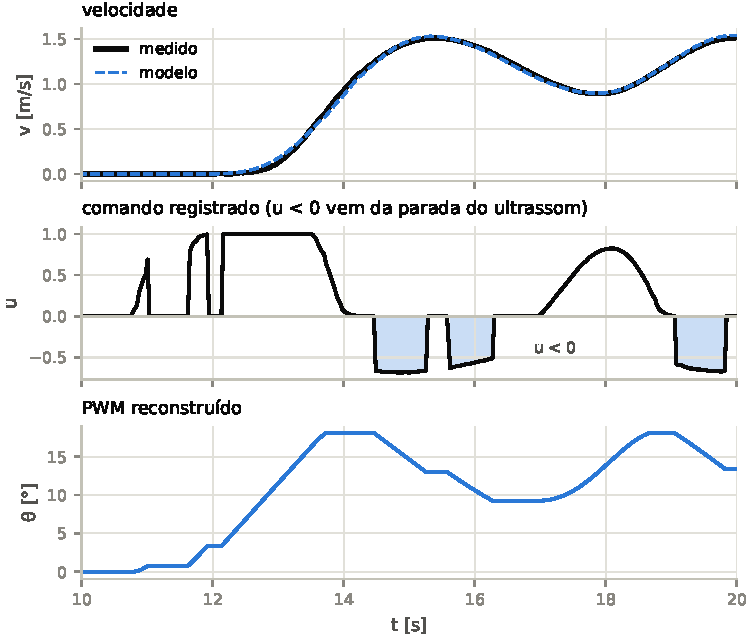
\includegraphics{pwm_desce}
  \caption{Ensaio 003552: $u < 0$ (área azul) baixa o PWM, e o carro desacelera. O modelo
  (azul tracejado) acompanha a descida e a subida.}
  \label{fig:desce}
\end{figure}

Um detalhe dessa figura voltará no projeto: ajustando constantes de tempo diferentes
para subir e para descer, a descida sai cerca de duas vezes mais lenta
($\tau \approx \SI{1,2}{s}$ contra \SI{0,6}{s}). Faz sentido: para acelerar, o motor
empurra; para desacelerar, só o atrito freia.

\subsection{Previsão cega --- e o erro de misturar condições}

O teste que realmente vale é prever um ensaio que o modelo não viu. O procedimento
\emph{deixa um de fora}: ajusta os parâmetros com todos os ensaios menos um e prevê o
que ficou de fora.

A primeira tentativa misturou todos os ensaios e falhou. A Tabela~\ref{tab:param} mostra
por quê: os parâmetros formam dois grupos. Das 00:26 às 00:33, $K \approx 1{,}5$--$1{,}6$
e $\tau \approx \SI{0,26}{s}$; a partir das 00:35, $K$ cai para $1{,}07$ e continua
caindo até $0{,}88$, enquanto $\tau$ sobe para 0,6--\SI{0,76}{s} (Figura~\ref{fig:bateria}).
É a bateria descarregando: tensão menor dá menos velocidade por grau de PWM (menor $G$),
e a resistência interna maior deixa o motor mais lento (maior $\tau$). Um modelo único não
pode prever os dois estados.

\begin{figure}[ht]
  \centering
  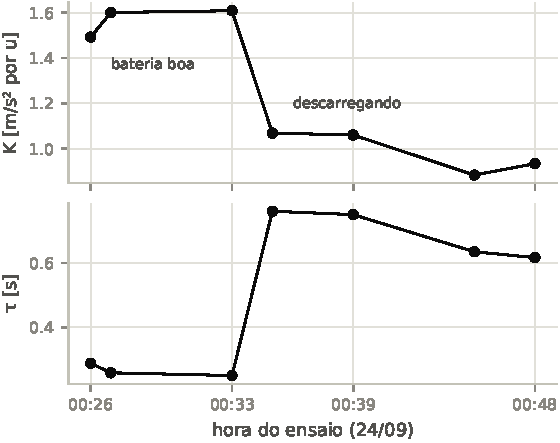
\includegraphics{bateria}
  \caption{Parâmetros ajustados ao longo da sessão. A planta muda com a carga da bateria.}
  \label{fig:bateria}
\end{figure}

Separando por estado da bateria:

\begin{center}\small
\begin{tabular}{llc}
\toprule
grupo & ensaio previsto & rmse da previsão cega [m/s]\\
\midrule
bateria boa & 002634 / 002751 / 003330 & 0,063 / 0,023 / 0,044\\
descarregando & 003552 / 003904 / 004516 / 004851 & 0,110 / 0,132 / 0,063 / 0,060\\
misturando os grupos & 003552 & 0,164\\
\bottomrule
\end{tabular}
\end{center}

Na bateria boa, a previsão erra de 2 a \SI{6}{cm/s}. No grupo que descarregava, o erro é
maior porque o próprio $K$ continuava caindo de um ensaio para o outro.

\begin{armadilha}
Nunca misture num ajuste só ensaios de condições diferentes --- rampa e pista plana no
simulador, bateria cheia e fraca aqui. O ajuste vira uma média que não descreve nenhuma
das condições, e a previsão cega falha. Antes de juntar ensaios, verifique se os
parâmetros ajustados \emph{separadamente} são parecidos.
\end{armadilha}

\subsection{O que os dados não conseguem dizer}

Todos os ensaios úteis começam com o carro parado e aceleram. Nesse tipo de ensaio, três
coisas atrasam a resposta da mesma maneira: a zona morta $DB$ (o carro demora a sair), a
constante de tempo $\tau$ (a velocidade demora a chegar) e o atraso puro $d$. Uma pode
fazer o papel da outra.

Para ver isso, fixamos $d$ em vários valores e ajustamos os outros três parâmetros com os
ensaios da bateria boa (Figura~\ref{fig:perfil}). O erro praticamente não muda
(\SIrange{0,030}{0,031}{m/s}), mas $\tau$ vai de \SI{0,29}{s} a \SI{0,01}{s}: o ajuste
troca inércia por atraso puro sem piorar. Os dados não distinguem os dois. O ganho $G$,
que define o patamar, é bem determinado; a \emph{forma} do transitório, não.

\begin{figure}[ht]
  \centering
  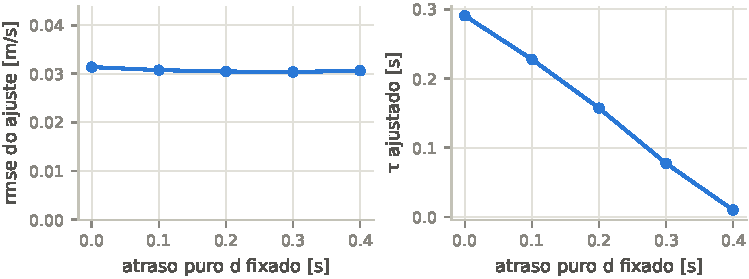
\includegraphics{perfil_tau_d}
  \caption{Perfil de custo: fixando o atraso puro $d$ e ajustando o resto. O erro fica
  plano enquanto $\tau$ despenca --- sinal de parâmetros não identificáveis com estes
  ensaios.}
  \label{fig:perfil}
\end{figure}

\begin{ideia}
Um parâmetro só é identificável se o ensaio o excita de um jeito que os outros parâmetros
não conseguem imitar. Para separar $\tau$ de $d$, seria preciso um ensaio em que o PWM
suba e desça várias vezes, em frequências diferentes. Enquanto isso não acontece, o
projeto precisa ser robusto a essa incerteza.
\end{ideia}

% ---------------------------------------------------------------------------
\section{Passo 7: perícia --- o que estava rodando no carro?}

Antes de concluir qualquer coisa sobre o controlador, é preciso saber \emph{qual}
controlador rodou. Nos ensaios, versões diferentes foram enviadas ao carro, e nem sempre o
envio funcionou. Os logs, porém, guardam tudo o que é preciso para descobrir: o $v$ e o
$v_{\text{ref}}$ que o controlador recebeu e o $u$ que ele respondeu.

O método: pegar a lei de controle candidata, alimentá-la com o $v$ e o $v_{\text{ref}}$
registrados, na mesma ordem da Figura~\ref{fig:laco}, e comparar o $u$ produzido com o
$u$ registrado. Se a lei for a mesma, a diferença é zero até o arredondamento. Durante a
parada do ultrassom, o controlador não roda (quem manda é o \code{set\_vel(0)}), então o
estado dele fica congelado nesses trechos.

\begin{center}\small
\begin{tabular}{lcc}
\toprule
ensaio & rmse, lei completa & rmse, lei sem o FF da referência\\
\midrule
002158 a 004516 (nove ensaios) & 0,0000 & 0,039 a 0,101\\
004851 & 0,0507 & 0,0000\\
\bottomrule
\end{tabular}
\end{center}

\begin{figure}[ht]
  \centering
  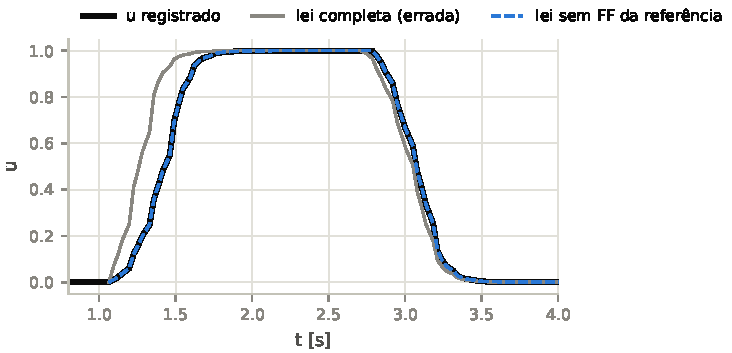
\includegraphics{pericia}
  \caption{Ensaio 004851: só a lei sem o \emph{feedforward} da referência reproduz o $u$
  registrado.}
  \label{fig:pericia}
\end{figure}

Resultado: até o 004516 rodou o controlador completo do simulador; no 004851, a versão sem
o \emph{feedforward} da referência. As outras variações testadas no código não chegaram a
rodar no carro. A Figura~\ref{fig:pericia} mostra a diferença: a lei certa se encaixa
perfeitamente, a errada não.

% ---------------------------------------------------------------------------
\section{Passo 8: um simulador do carro real}

Testar cada ganho no carro é lento, gasta bateria e --- como vimos --- a bateria muda a
planta. Com o modelo identificado, dá para montar um simulador do carro real e fazer o
projeto nele. Para ser útil, ele precisa reproduzir o carro também \emph{em malha
fechada}, então inclui tudo o que afeta o laço:
\begin{itemize}\itemsep0pt
  \item a planta~\eqref{eq:modelo-real} com os parâmetros da Tabela~\ref{tab:param};
  \item a média de 30 amostras e a proteção do \code{set\_u} ($|v| > \SI{1,5}{m/s}
    \Rightarrow u = 0$), mais a saturação $u\in[-1,1]$;
  \item o período do laço sorteado da distribuição real (Figura~\ref{fig:dt}) e o
    \SI{1}{s} parado do \code{start\_mission};
  \item a ordem de operações da Figura~\ref{fig:laco}.
\end{itemize}

A validação: rodar no simulador o controlador \emph{antigo}, o mesmo que rodou no carro, e
comparar com os ensaios (Figura~\ref{fig:malha}).

\begin{center}\small
\begin{tabular}{lcccc}
\toprule
& \multicolumn{2}{c}{velocidade final [m/s]} & \multicolumn{2}{c}{tempo com $u=1$ [s]}\\
\cmidrule(lr){2-3}\cmidrule(lr){4-5}
ensaio & simulador & carro & simulador & carro\\
\midrule
003330 (bateria boa, $v_{\text{ref}} = 1$) & 1,88 & 1,85 & 1,02 & 0,99\\
003904 (descarregando, $v_{\text{ref}} = 1$) & 1,74 & 1,75 & 1,44 & 1,49\\
004516 (mais fraca, $v_{\text{ref}} = 0{,}5$) & 1,28 & 1,31 & 0,94 & 0,96\\
\bottomrule
\end{tabular}
\end{center}

\begin{figure}[ht]
  \centering
  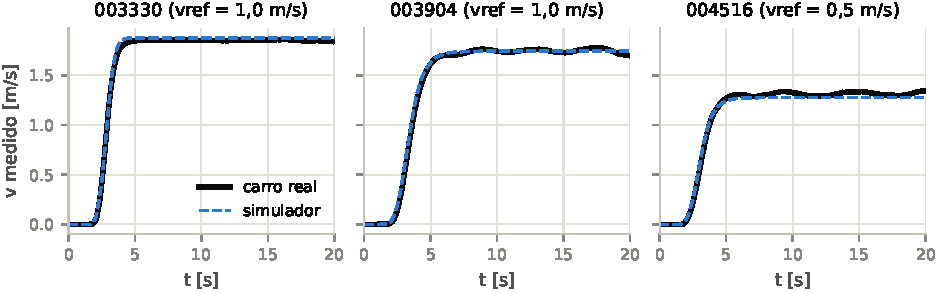
\includegraphics{validacao_malha}
  \caption{O simulador de malha fechada com o controlador antigo reproduz a catraca vista
  nos ensaios.}
  \label{fig:malha}
\end{figure}

\begin{armadilha}
Esta validação não é cega: a planta foi ajustada nesses mesmos ensaios. O que ela prova é
que a \emph{montagem} da malha está certa --- período do laço, média móvel, ordem das
operações, saturações. A validação cega do simulador só vem com o primeiro ensaio do
controlador novo no carro.
\end{armadilha}

% ---------------------------------------------------------------------------
\section{Passo 9: projete o controlador}

\subsection{A estrutura sai da planta}

Cada termo do controlador do simulador existia por causa de algo na planta do simulador.
A planta real é outra, então cada termo precisa ser revisto com a mesma pergunta: o que
na planta justifica este termo?

\begin{center}\small
\begin{tabularx}{\textwidth}{>{\raggedright\arraybackslash}p{3.2cm}>{\raggedright\arraybackslash}p{2.8cm}X}
\toprule
no simulador & no carro real & por quê\\
\midrule
PI & só P &
A planta já tem um integrador (o PWM). Com só P, a malha é do tipo 1 e já tem erro zero em
regime (ver abaixo). O I tornaria a malha do tipo 2: $-90^\circ$ a mais de fase em baixa
frequência, mais sobressinal e \emph{windup}, sem ganhar nada em regime.\\
\addlinespace
compensação de atrito $a_0$, $c$ & removida &
Medido no Passo 6: com $u = 0$ a velocidade fica parada. O atrito já está dentro da curva
PWM$\to v$. O termo vira um viés de $\approx 0{,}1$ em $u$ (ver abaixo).\\
\addlinespace
$u \in [0,\,1]$ & $u \in [-1,\,1]$ &
$u < 0$ é o único jeito de baixar o acelerador. Com $u \ge 0$, a catraca do Passo 4.\\
\addlinespace
filtro passa-baixas em $u$ & removido &
O integrador do PWM já filtra $u$; o filtro só somava atraso.\\
\addlinespace
FF da referência & mantido, dividido por $\Knom$ &
Para seguir uma rampa de inclinação $a$, o integrador precisa de $u = a/K$: é a inversão
do modelo.\\
\addlinespace
erro $= v_{\text{des}} - \vmed$ & erro $= \mathrm{MA30}(v_{\text{des}}) - \vmed$ &
A medição chega \SI{0,42}{s} atrasada; a referência precisa do mesmo atraso
(Seção~\ref{sec:casada}).\\
\bottomrule
\end{tabularx}
\end{center}

\paragraph{Por que só P basta.} Chame de $P_2(s)$ tudo o que vem depois do integrador do
PWM (zona morta linearizada, ganho, inércia). Com um controlador proporcional $K_P$ e uma
perturbação constante $\delta$ somada \emph{depois} do integrador --- a bateria cedendo, uma
subida, a zona morta ---, o erro é
\begin{equation}
  E(s) = \frac{s}{s + k_\theta K_P P_2(s)}\big(R(s) - P_2(s)\,\Delta(s)\big).
\end{equation}
O fator $s$ no numerador vem do integrador do PWM. Pelo teorema do valor final, o erro
em regime é zero tanto para uma referência em degrau quanto para uma perturbação em
degrau. O integral do PI não acrescenta nada aqui.

\paragraph{Por que a compensação de atrito atrapalha.} O raciocínio vale ao contrário
para um viés $b$ somado \emph{antes} do integrador, direto em $u$. Em regime, o PWM só
para se a entrada do integrador for zero, ou seja, $K_P e/\Knom + b = 0$:
\begin{equation}
  e_{ss} = -\,\frac{b\,\Knom}{K_P}.
\end{equation}
A compensação de atrito é exatamente um viés desses, $b \approx 0{,}1$. Com os ganhos que
vamos escolher, ela deixaria um erro de regime de cerca de \SI{0,27}{m/s}. O simulador do
Passo 8 confirma: somando $b = 0{,}1$ ao controlador escolhido, o erro de regime medido é de
$-\SI{0,267}{m/s}$, o mesmo valor da fórmula. A compensação existia para cancelar um atrito
que, no carro real, não aparece na entrada.

\subsection{O atraso do sensor e a referência casada}
\label{sec:casada}

A Figura~\ref{fig:fase} compara a fase da média de 30 amostras com o atraso de
\SI{0,05}{s} que o projeto do simulador assumia. A \SI{1}{rad/s}, a média já consome
$24^\circ$; a \SI{4}{rad/s}, a banda do projeto antigo, consome $95^\circ$, contra
$11^\circ$ do atraso do simulador. Só isso já explica por que os ganhos do simulador não
servem: com eles ($K_P = 4$, $K_I = 2{,}67$ e o filtro de \SI{0,1}{s} em $u$), a malha real
cruzaria \SI{0}{dB} em \SI{3,3}{rad/s} com margem de fase de $-64^\circ$ na bateria boa
($-50^\circ$ na fraca). Seria instável.

\begin{figure}[ht]
  \centering
  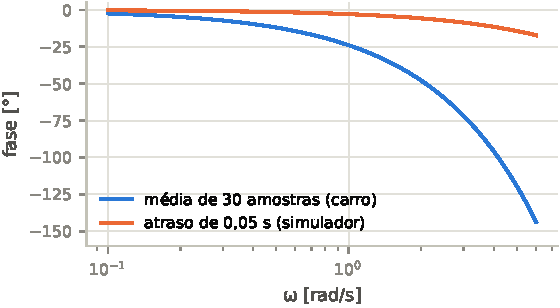
\includegraphics{fase_ma}
  \caption{Fase introduzida pela média móvel de 30 amostras no carro (período de
  \SI{28,8}{ms}) e pelo atraso de \SI{0,05}{s} considerado no simulador. O eixo para em
  \SI{6}{rad/s} porque em $2\pi/(NT) \approx \SI{7,3}{rad/s}$ a média tem seu primeiro
  zero: ela anula por completo um sinal nessa frequência.}
  \label{fig:fase}
\end{figure}

O atraso também atrapalha o seguimento da rampa. Se o erro for
$v_{\text{des}} - \vmed$, durante uma rampa de \SI{0,9}{m/s^2} a velocidade medida fica
$0{,}9 \times 0{,}42 \approx \SI{0,38}{m/s}$ abaixo da real, só por causa do sensor. O
controlador ``vê'' esse erro, acelera a mais e passa da referência.

A solução é passar a referência pela \emph{mesma} média móvel antes de compará-la com a
medição (Figura~\ref{fig:dof}). Os dois lados do erro ficam com o mesmo atraso, e o
proporcional só reage ao erro real. Isso é um controlador de \emph{dois graus de
liberdade}: o caminho da referência (rampa, filtro, FF, média) é separado do caminho da
realimentação ($K_P$). A referência fica fora da malha, então essa mudança não mexe na
estabilidade; só melhora a resposta à referência.

\begin{figure}[ht]
\centering
\begin{tikzpicture}[>={Stealth}, node distance=4mm and 5mm, font=\footnotesize,
  bl/.style={draw=azul, fill=azul!10, rounded corners=2pt, align=center, minimum height=9mm, inner sep=2pt},
  hl/.style={bl, fill=azul!28},
  pl/.style={draw=cinza, fill=cinza!10, rounded corners=2pt, align=center, minimum height=9mm, inner sep=2pt},
  sm/.style={draw, circle, inner sep=1.2pt}]
  \node (r) {$v_{\text{ref}}$};
  \node[bl, right=of r] (ramp) {rampa\\\SI{0,9}{m/s^2}};
  \node[bl, right=of ramp] (lpf) {passa-baixas\\$\tau_v = \SI{0,3}{s}$};
  \node[hl, right=13mm of lpf] (ma1) {média\\de 30};
  \node[sm, right=of ma1] (s1) {$\Sigma$};
  \node[bl, right=of s1] (kp) {$K_P$};
  \node[sm, right=of kp] (s2) {$\Sigma$};
  \node[bl, right=of s2] (k) {$\div\Knom$\\sat $\pm1$};
  \node[pl, right=6mm of k] (car) {carro};
  \node[bl, above=5mm of ma1] (dd) {$\dfrac{d}{dt}$\\(do filtro)};
  \node[pl, below=6mm of car] (ma2) {média de 30\\\scriptsize\code{car.py}};
  \draw[->] (r) -- (ramp);
  \draw[->] (ramp) -- (lpf);
  \draw[->] (lpf) -- node[below, pos=0.45] {$v_{\text{des}}$} (ma1);
  \draw[->] ($(lpf.east)!0.45!(ma1.west)$) |- (dd.west);
  \draw[->] (dd.east) -| node[above, pos=0.25] {FF} (s2.north);
  \draw[->] (ma1) -- node[above, pos=0.35] {$+$} (s1);
  \draw[->] (s1) -- node[above] {$e$} (kp);
  \draw[->] (kp) -- (s2);
  \draw[->] (s2) -- (k);
  \draw[->] (k) -- node[above] {$u$} (car);
  \draw[->] (car.south) -- (ma2.north);
  \draw[->] (ma2.west) -| node[below, pos=0.3] {$\vmed$} node[right, pos=0.93] {$-$} (s1.south);
\end{tikzpicture}
\caption{O controlador novo. A referência passa pela mesma média de 30 amostras que a
medição (bloco destacado), e o \emph{feedforward} vem da derivada da referência filtrada.}
\label{fig:dof}
\end{figure}

A Figura~\ref{fig:casada} mostra o efeito, no simulador, com o mesmo $K_P$. O erro não
some: a zona morta e a inércia continuam atrasando o carro em relação à referência, e isso
é erro de verdade, que o proporcional precisa corrigir. O casamento remove só a parte que
era atraso do sensor. O pico do erro cai de 0,80 para \SI{0,59}{m/s} e, mais
importante, o erro quase não fica negativo depois da rampa ($-0{,}014$ contra
$-\SI{0,079}{m/s}$). Esse trecho negativo é o controlador corrigindo um sobressinal que ele
mesmo causou por ter acelerado a mais. Sem ele, o sobressinal cai de 8,2\% para 1,5\%.

\begin{figure}[ht]
  \centering
  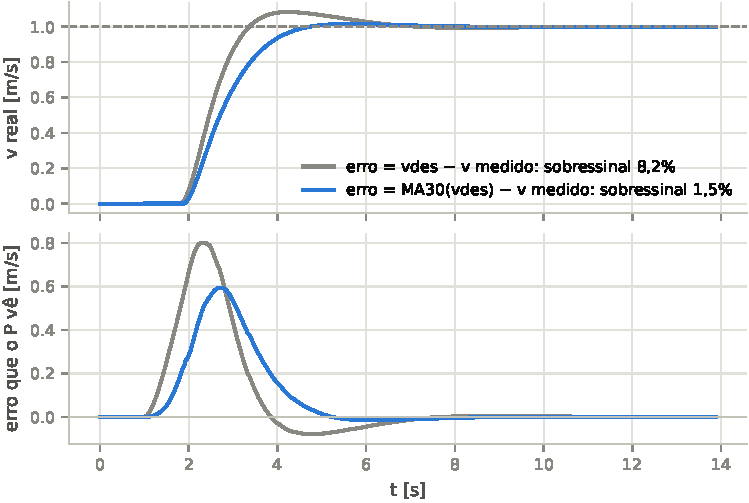
\includegraphics{referencia_casada}
  \caption{Com a referência casada (azul), o erro que o proporcional vê deixa de incluir o
  atraso do sensor: o pico cai e o trecho negativo depois da rampa quase some.}
  \label{fig:casada}
\end{figure}

\subsection{O ganho nominal $\Knom$}

A lei de controle é
\begin{equation}
  u = \mathrm{sat}_{\pm1}\!\left(\frac{K_P\,\big(\mathrm{MA30}(v_{\text{des}}) - \vmed\big)
      + \dot v_{\text{des}}}{\Knom}\right).
  \label{eq:lei}
\end{equation}
$\Knom$ é a estimativa de $K$ que o controlador usa para converter aceleração desejada em
$u$. O \emph{feedforward} $\dot v_{\text{des}}/\Knom$ só acerta a rampa se $\Knom = K$.

Com a premissa de trabalho de que a bateria estará sempre carregada, a planta de projeto é
a do grupo da bateria boa: $K = 1{,}49$, $1{,}60$ e $1{,}61$ nos três ensaios. Daí
$\Knom = 1{,}6$. Se o $K$ real for diferente, duas coisas acontecem:
\begin{itemize}\itemsep0pt
  \item o \emph{feedforward} erra a aceleração da rampa na mesma proporção, e o
    proporcional corrige o resto;
  \item o ganho de malha vira $K_P\,K/\Knom$: com $K$ maior, a malha fica mais rápida e
    com menos margem; com $K$ menor, mais lenta e com mais margem.
\end{itemize}
Por isso o projeto é verificado com $K$ de 1,3 a 2,0. O limite de cima não é exagero: a
``bateria boa'' dos ensaios não estava cheia --- perdeu 34\% de $G$ em cerca de um minuto
de uso ---, então uma bateria cheia de verdade pode ter $K$ acima de 1,6.

\subsection{O ganho $K_P$}

Com a lei~\eqref{eq:lei} e a planta~\eqref{eq:modelo-real} linearizada acima da zona
morta, a função de transferência de malha aberta é
\begin{equation}
  L(s) = \frac{K_P}{\Knom}\,K\;\frac{\mathrm{MA30}(s)\;e^{-0{,}03 s}}{s\,(\tau s + 1)}.
  \label{eq:L}
\end{equation}
Três observações guiam a escolha:
\begin{itemize}\itemsep0pt
  \item com $K = \Knom$ e sem os atrasos, $L(s) = K_P/s$: um integrador cujo ganho cruza
    \SI{0}{dB} em $\omega = K_P$. Por isso $K_P$ tem unidade de rad/s: \emph{ele é a banda
    da malha};
  \item a média móvel tem fase $-\omega \cdot \SI{0,42}{s}$: quanto maior a banda, mais
    fase ela come no cruzamento;
  \item o termo $e^{-0{,}03s}$ é uma margem para a janela do encoder (cerca de
    \SI{15}{ms}) e o período da thread do atuador (cerca de \SI{15}{ms}). Os ajustes deram
    $d \approx 0$, absorvido em $\tau$; os \SI{30}{ms} ficam por segurança.
\end{itemize}

A Figura~\ref{fig:bode} mostra $L(j\omega)$ para $K_P = 0{,}6$ no caso nominal, com e sem
a média móvel. Sem ela, a margem seria confortável; com ela, a fase cai rápido acima de
\SI{1}{rad/s}.

\begin{figure}[ht]
  \centering
  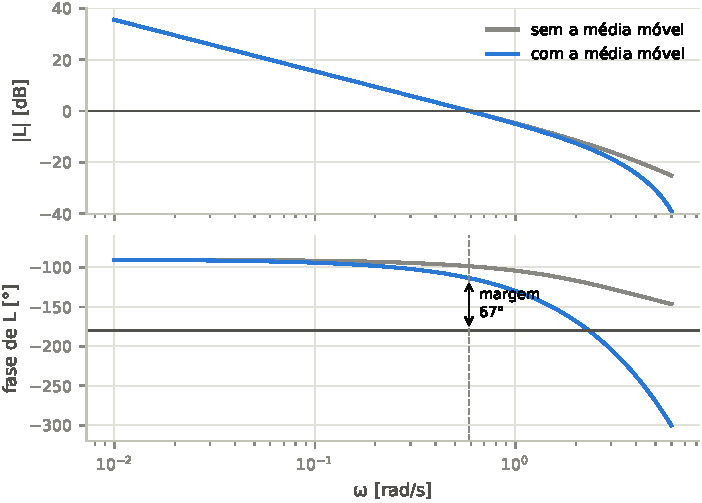
\includegraphics{bode_L}
  \caption{Diagrama de Bode da malha aberta com $K_P = 0{,}6$ (caso nominal: $K = 1{,}6$,
  $\tau = \SI{0,25}{s}$). A média móvel é o que limita a margem.}
  \label{fig:bode}
\end{figure}

\paragraph{Critério 1: margem de fase no pior caso plausível.} A Tabela~\ref{tab:pm} e a
Figura~\ref{fig:pmkp} dão a margem de fase para vários $K_P$ e plantas. O pior caso é
$K$ alto com $\tau$ alto: $K$ alto leva o cruzamento para frequências onde a fase da média
cai rápido, e $\tau$ alto soma atraso na mesma frequência.

\begin{table}[ht]
\centering\small
\caption{Margem de fase [graus] da malha~\eqref{eq:L}, com $\Knom = 1{,}6$.}
\label{tab:pm}
\begin{tabular}{cccccc}
\toprule
$K_P$ & nominal ($K$ 1,6, $\tau$ 0,25) & $K$ 2,0 & $K$ 1,3 & $\tau$ 0,40 & $K$ 2,0 e $\tau$ 0,40\\
\midrule
0,4 & 74,2 & 70,3 & 77,1 & 71,0 & 66,5\\
\rowcolor{azul!6}0,6 & 66,6 & 61,1 & 70,8 & 62,1 & 55,9\\
0,8 & 59,3 & 52,4 & 64,7 & 53,9 & 46,4\\
1,0 & 52,4 & 44,3 & 58,8 & 46,4 & 38,0\\
1,2 & 45,9 & 36,9 & 53,2 & 39,6 & 30,5\\
\bottomrule
\end{tabular}
\end{table}

\begin{figure}[ht]
  \centering
  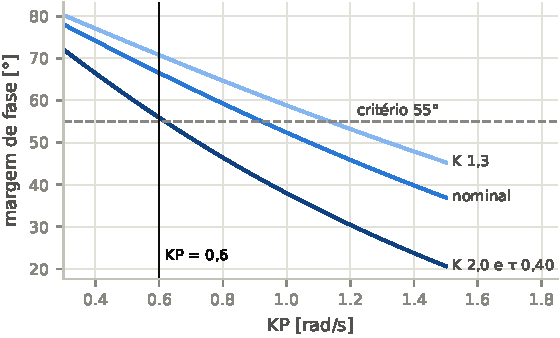
\includegraphics{margem_kp}
  \caption{Margem de fase em função de $K_P$ para três plantas. O critério de
  \SI{55}{\degree} no pior caso limita $K_P$ a 0,6.}
  \label{fig:pmkp}
\end{figure}

\paragraph{Critério 2: resposta no tempo, no simulador não linear.} A margem de fase é
uma análise linear; o carro tem zona morta, saturação do PWM, saturação de $u$, período
variável e desaceleração mais lenta que a aceleração (Seção~\ref{sec:desce}). Todos esses
efeitos estão no simulador do Passo 8. Para cada $K_P$, a Tabela~\ref{tab:tempo} mostra o
pior resultado entre $v_{\text{ref}} = 1{,}0$ e $0{,}5$ e o tempo para voltar a menos de
5\% da referência depois de uma queda súbita de 20\% no ganho da planta (bateria cedendo
ou início de uma subida).

\begin{table}[ht]
\centering\small
\caption{Resposta no tempo no simulador do carro real (desaceleração 2 vezes mais lenta
que a aceleração). A acomodação é contada desde o início da missão e inclui cerca de
\SI{1}{s} parado no \code{start\_mission}.}
\label{tab:tempo}
\begin{tabular}{lccccc}
\toprule
& \multicolumn{3}{c}{sobressinal} & acomodação & volta após\\
\cmidrule(lr){2-4}
$K_P$ & nominal & $K$ 2,0 & pior caso & nominal & queda de 20\%\\
\midrule
\rowcolor{azul!6}0,6 & 1,5\% & 7,9\% & 14,0\% & \SI{5,0}{s} & \SIrange{2,7}{3,8}{s}\\
0,8 & 7,6\% & 16,4\% & 23,5\% & \SI{5,9}{s} & \SIrange{2,3}{3,0}{s}\\
1,0 & 15,4\% & 26,0\% & 33,8\% & \SI{5,7}{s} & \SIrange{2,0}{2,6}{s}\\
\midrule
0,6 (sem casar) & 8,2\% & 22,7\% & 27,7\% & \SI{5,4}{s} & \SIrange{2,7}{3,8}{s}\\
\bottomrule
\end{tabular}
\end{table}

\begin{figure}[ht]
  \centering
  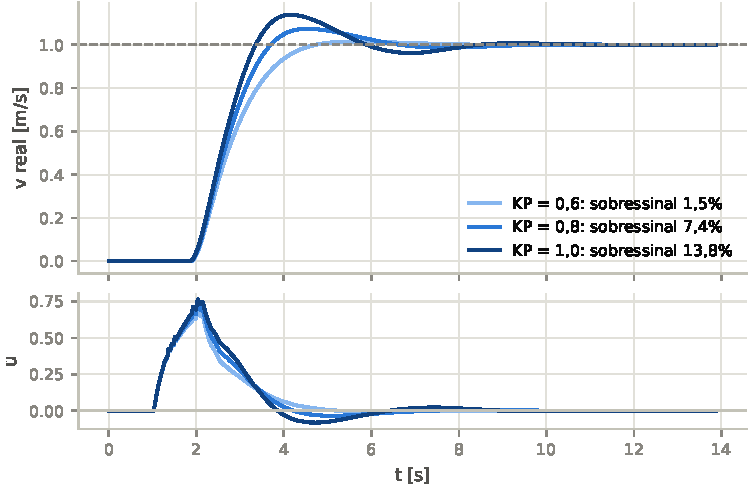
\includegraphics{resposta_kp}
  \caption{Resposta à rampa de referência até \SI{1}{m/s} no caso nominal, com a
  desaceleração 2 vezes mais lenta que a aceleração. Acima de $K_P = 0{,}6$, o
  sobressinal cresce rápido, porque o atraso da média domina. (A figura mostra
  $v_{\text{ref}} = 1$; a Tabela~\ref{tab:tempo} traz o pior caso entre
  $v_{\text{ref}} = 1$ e $0{,}5$, por isso seus números são um pouco maiores.)}
  \label{fig:resposta}
\end{figure}

\paragraph{A escolha.} O critério foi: o maior $K_P$ com sobressinal nominal de no máximo
cerca de 2\% e margem de fase de pelo menos \SI{55}{\degree} no pior caso. O resultado é
$K_P = \SI{0,6}{rad/s}$. Subir $K_P$ recupera perturbações cerca de \SI{1}{s} mais rápido,
mas o sobressinal cresce depressa (Figura~\ref{fig:resposta}). Descer deixa a recuperação
mais lenta.

\subsection{Robustez}

A Figura~\ref{fig:robustez} mostra o controlador escolhido com três valores de $K$. Com
$K$ menor (bateria cedendo), a resposta fica mais lenta e sem sobressinal; com $K$ maior
(bateria mais cheia que a dos ensaios), aparece algum sobressinal, sem oscilar. Com as
plantas da bateria que descarregava (ajustes próprios dos ensaios 003904 e 004516, com
$K = 1{,}06$ e $0{,}88$), o controlador ainda acomoda, só mais devagar: sobressinal de 0,2
a 4\% e acomodação em \SIrange{5,5}{6,6}{s}.

\begin{figure}[ht]
  \centering
  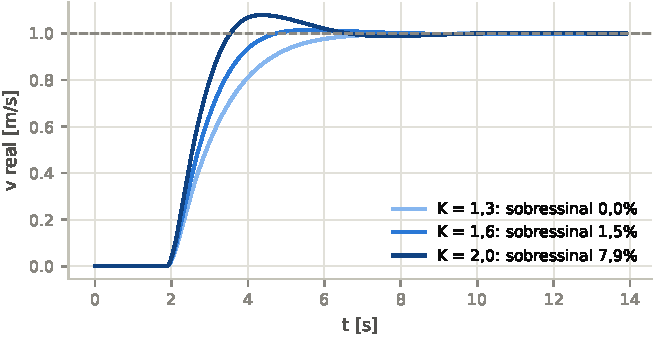
\includegraphics{robustez}
  \caption{Controlador final ($K_P = 0{,}6$, $\Knom = 1{,}6$) com $K = 1{,}3$, $1{,}6$ e
  $2{,}0$.}
  \label{fig:robustez}
\end{figure}

\subsection{Verificar a implementação}

O projeto foi feito com uma versão do controlador escrita para o simulador. O que vai para
o carro é o código em \code{veiculo\_real/main.py}. Para garantir que os dois são a mesma
coisa, o \code{figuras.py} carrega o \code{main.py} de verdade (trocando as bibliotecas de
hardware por módulos falsos), roda o \code{control\_func} dele dentro do simulador e
compara com a versão de projeto: a diferença máxima em $u$ é da ordem de $10^{-16}$,
arredondamento de ponto flutuante.

\needspace{17\baselineskip}
\begin{lstlisting}[title={\small\code{veiculo\_real/main.py} (trecho do controlador)}]
def controlador_longitudinal(car, vdes_bruto):
    if car.dt > 0:
        _vdes_filt.alpha = np.clip(car.dt / TAU_VDES, 0.0, 1.0)
    vdes_anterior = _vdes_filt.value
    vdes = _vdes_filt.filter(vdes_bruto)
    feedforward_dvdes = (vdes_bruto - vdes_anterior) / TAU_VDES

    vdes_ma = _estado.setdefault('vdes_ma', MovingAverage(n=car.v_filt.n))
    erro = vdes_ma.filter(vdes) - car.v

    u = (KP_MOD * erro + feedforward_dvdes) / K_NOM
    return float(np.clip(u, -1.0, 1.0))
\end{lstlisting}

A Figura~\ref{fig:antesdepois} fecha o capítulo: o mesmo carro simulado com o controlador
antigo e com o novo.

\begin{figure}[ht]
  \centering
  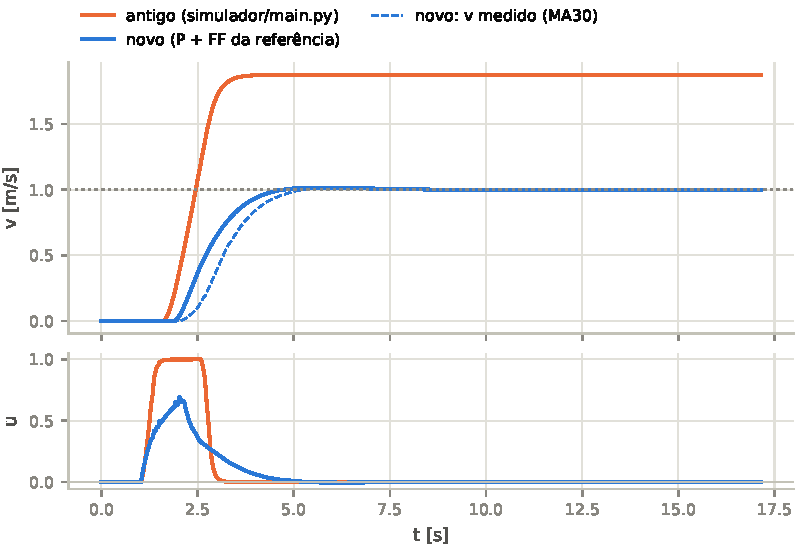
\includegraphics{antes_depois}
  \caption{Controlador antigo e novo no simulador do carro real (bateria carregada). O
  antigo trava o acelerador; o novo chega a \SI{1}{m/s} com cerca de 1,5\% de sobressinal
  e usa $u<0$ para devolver o acelerador.}
  \label{fig:antesdepois}
\end{figure}

% ---------------------------------------------------------------------------
\section{O que ainda é hipótese}

Um projeto honesto termina listando o que ainda não foi provado:
\begin{itemize}\itemsep0pt
  \item \textbf{a bateria de projeto não estava cheia.} Uma bateria cheia pode ter $K$ acima
    de 1,6. A robustez cobre até 2,0;
  \item \textbf{$\tau$ e $d$ não foram separados} (Figura~\ref{fig:perfil}). O projeto
    considera $\tau$ até \SI{0,4}{s} e \SI{30}{ms} de atraso extra;
  \item \textbf{o simulador não foi validado às cegas.} O primeiro ensaio do controlador
    novo no carro cumpre esse papel. Com bateria carregada e $v_{\text{ref}} = \SI{1}{m/s}$,
    a previsão é que a velocidade chegue a \SI{1}{m/s} cerca de \SI{3}{s} depois do início da
    rampa, sem passar de \SI{1,02}{m/s}. Se passar muito disso, aquela bateria tem outro $K$
    ou outro $\tau$ --- e o log desse ensaio é exatamente o dado para reidentificar;
  \item \textbf{o atraso da média de 30 amostras é o maior limitante.} Pela variação da
    saída da média em regime, o ruído do encoder bruto é da ordem de \SI{0,03}{m/s}. Se isso
    se confirmar registrando o encoder sem filtro, uma média bem mais curta cortaria a maior
    parte do atraso e permitiria um $K_P$ bem maior.
\end{itemize}

% ---------------------------------------------------------------------------
\section{Resumo do método}

\begin{caixa}{O método em nove passos}
\begin{enumerate}\itemsep1pt
  \item \textbf{Código antes de dados.} Siga o comando até o atuador e a medição até o
    controlador. Tudo o que o código determina não é parâmetro: é estrutura.
  \item \textbf{Modele só o resto}, com poucos parâmetros e significado físico.
  \item \textbf{Faça inventário} (cópias, período real do laço) e \textbf{triagem com
    evidência} (IMU, comando, referência).
  \item \textbf{Reconstrua} os sinais internos que o código permite calcular.
  \item \textbf{Ajuste por erro de saída}: o modelo recebe só a entrada e prevê a
    trajetória inteira.
  \item \textbf{Valide}: um teste físico (o que acontece com $u = 0$?), um ensaio com
    excitação diferente, previsão cega sem misturar condições e um perfil de custo para
    ver o que não é identificável.
  \item \textbf{Descubra o que rodou}, reproduzindo o comando registrado.
  \item \textbf{Monte um simulador de malha fechada} e valide-o contra os ensaios.
  \item \textbf{Projete a partir da planta}: cada termo do controlador precisa de uma
    razão na planta; os ganhos saem de um critério na frequência (margem no pior caso) e
    de um no tempo (sobressinal, acomodação, recuperação de perturbação).
\end{enumerate}
\end{caixa}

% ---------------------------------------------------------------------------
\section{Exercícios}

\begin{enumerate}
  \item Calcule o atraso de grupo de uma média móvel de 10 amostras a \SI{28,8}{ms}. Refaça
    a Tabela~\ref{tab:pm} com essa média no lugar da MA30 (use o \code{figuras.py}). Qual
    o maior $K_P$ com margem de \SI{55}{\degree} no pior caso?
  \item Mostre que, com um controlador PI em vez de P, a malha~\eqref{eq:L} passa a ter dois
    integradores. Desenhe o diagrama de Bode de fase em baixa frequência e explique por que
    isso reduz a margem de fase para a mesma banda.
  \item Com a lei~\eqref{eq:lei} e a compensação de atrito somada ($b = 0{,}1$), use o
    simulador para medir o erro de regime. Compare com $e_{ss} = -b\,\Knom/K_P$.
  \item Projete um ensaio que separe $\tau$ de $d$. Que sinal de $u$ você usaria? Por quanto
    tempo? Como saberia, antes de rodar, que ele excita a diferença entre os dois?
  \item No ensaio 003552, ajuste constantes de tempo separadas para subir e para descer.
    Use o resultado no simulador e verifique se a escolha de $K_P$ muda.
  \item A proteção do \code{set\_u} faz $u = 0$ quando $|v| > \SI{1,5}{m/s}$. Neste carro,
    o que essa proteção faz com o acelerador? Proponha uma alteração de uma linha que a
    torne efetiva e justifique com a equação~\eqref{eq:integrador}.
\end{enumerate}

% ---------------------------------------------------------------------------
\section*{Como reproduzir}

Todos os números e figuras deste capítulo saem de um único script, o
\code{figuras.py}, que lê os logs da pasta
\path{veiculo_real/dados2_sem_feedforward/roxo}:
\begin{lstlisting}[language=bash]
simulador/.venv/Scripts/python.exe veiculo_real/capitulo/figuras.py
cd veiculo_real/capitulo
pdflatex -aux-directory=build controle_carro_real.tex    # duas vezes
\end{lstlisting}

\end{document}
